\documentclass[12pt,a4paper]{ctexart}

\usepackage[margin=2.4cm]{geometry}
\usepackage{graphicx}
\usepackage{booktabs}
\usepackage{float}
\usepackage{amsmath}
\usepackage{array}
\usepackage{caption}
\usepackage{subcaption}
\usepackage{xcolor}
\usepackage[sort&compress]{gbt7714}
\usepackage[hidelinks]{hyperref}
\emergencystretch=3em

\title{家庭电力消耗多变量时间序列预测}
\author{作者：侯嘉睿 \quad 研究领域：机器学习与智能电力负荷预测}
\date{2026 年 6 月}

\begin{document}
\maketitle

\noindent\textbf{Github 链接：} \url{https://github.com/RxHou/ml_power_forecast}

\section{问题介绍}

随着智能家居与物联网技术的发展，家庭电力消耗监测与预测可以帮助居民理解自身用电行为、发现异常用电，并为电力公司负荷调度和供需平衡提供参考。本实验以 UCI 家庭电力消耗数据和 Météo-France 月度气象数据为主要数据基础\cite{uci,meteofrance-monthly}。家庭用电受到季节、日期、生活习惯、电器使用模式和天气等多种因素影响，具有明显的时间依赖和波动性，因此适合建模为多变量时间序列预测问题。已有研究也将深度学习用于住宅负荷预测和多步时间序列预测，说明该问题不仅是传统回归任务，也适合用序列模型刻画时序依赖\cite{residential-lstm,tft}。

本实验使用 UCI Machine Learning Repository 公开的 Individual Household Electric Power Consumption 数据集\cite{uci}。该数据记录了法国 Sceaux 附近一户家庭从 2006 年 12 月 16 日至 2010 年 11 月 26 日的分钟级用电情况，包括全局有功功率、无功功率、电压、电流强度以及三个分表能耗。原始数据共有 2,075,259 条记录，其中存在 25,979 条缺失记录。根据课程要求，本实验将分钟级数据聚合为天级数据，共得到 1,442 天样本。

为满足作业中融合天气因素的要求，本实验进一步引入 data.gouv.fr 上由 Météo-France 发布的月度基础气象数据\cite{meteofrance-monthly}。最终选择的数据文件为 \path{MENS_departement_75_periode_1950-2024}，对应下载文件为 \path{MENSQ_75_previous-1950-2024.csv.gz}；具体站点为 \path{NUM_POSTE=75114001} 的 \texttt{PARIS-MONTSOURIS}。选择该站点的原因是：UCI 数据家庭位于 Sceaux，距巴黎约 7 km，而 Paris-Montsouris 距 Sceaux 约 5.9 km，空间上较接近；同时该站在 2006 年 12 月至 2010 年 11 月期间对 \texttt{RR}、\texttt{NBJRR1}、\texttt{NBJRR5}、\texttt{NBJRR10}、\texttt{NBJBROU} 均有完整月度记录。相比之下，虽然 92 省行政区更贴近 Sceaux，但其站点在所需字段或时间覆盖上缺失更多，因此没有作为最终天气来源。

电力数据聚合时，\path{global_active_power}、\path{global_reactive_power} 以及三个分表能耗字段按天求和，\texttt{voltage} 和 \path{global_intensity} 按天求平均。缺失日期通过时间插值并结合前向、后向填充处理。另根据课程提示计算剩余分表能耗：
\begin{align*}
\text{sub\_metering\_remainder} &=
\text{global\_active\_power}\times \frac{1000}{60}\\
&\quad - (\text{sub\_metering\_1}
+\text{sub\_metering\_2}
+\text{sub\_metering\_3}).
\end{align*}
气象数据按月份与日级样本对齐：先用每一天所在月份构造 \texttt{AAAAMM}，再与 Paris-Montsouris 的月度气象记录连接。字段 \texttt{RR} 原始单位为 0.1 mm，本实验除以 10 后得到月降水量 \texttt{weather\_rr\_mm}；\texttt{NBJRR1}、\texttt{NBJRR5}、\texttt{NBJRR10} 和 \texttt{NBJBROU} 分别表示当月降水量不小于 1 mm、5 mm、10 mm 的天数以及雾日数。最终输入特征包括 8 个电力与能耗特征、4 个星期和一年中日期的正余弦编码特征，以及 5 个天气特征，共 17 个变量。

预测任务为：基于过去 90 天的多变量特征，分别预测未来 90 天和未来 365 天的每日总有功功率。两个预测长度分别训练独立模型，避免短期和长期任务之间共享模型参数。数据集按时间顺序构造滑动窗口，最后 20\% 窗口作为测试集，其余窗口再划分训练集和验证集。所有划分均保持时间顺序，避免随机划分造成未来信息泄漏。

\section{模型}

\subsection{LSTM 模型}

LSTM 通过门控机制缓解普通循环神经网络在长序列上的梯度衰减问题，适合建模用电序列中的顺序依赖\cite{lstm}。在住宅负荷预测任务中，已有研究表明 LSTM 能较好处理家庭负荷的短期波动\cite{residential-lstm}。本实验将过去 90 天的多变量输入送入两层 LSTM，取最后一层最后时刻的隐藏状态作为历史序列表示，再经过多层感知机一次性输出未来 $H$ 天的预测结果，其中 $H\in\{90,365\}$。

\begin{verbatim}
X = past 90-day multivariate sequence
h = LSTM(X).last_hidden_state
y_hat = MLP(h)
\end{verbatim}

\subsection{Transformer 模型}

Transformer 使用自注意力机制建模不同时间位置之间的依赖关系\cite{attention}。近年的 Informer、Autoformer、PatchTST 等工作进一步将 Transformer 思路扩展到长序列预测问题\cite{informer,autoformer,patchtst}。实验中先将每日特征线性映射到隐藏维度，再加入正弦位置编码，通过 Transformer Encoder 得到时间序列表示。最后对时间维度进行平均池化，并使用全连接层输出未来功率曲线。

\begin{verbatim}
Z = Linear(X) + PositionalEncoding
E = TransformerEncoder(Z)
h = MeanPool(E)
y_hat = MLP(h)
\end{verbatim}

\subsection{改进模型：CNN-Transformer}

自提出模型采用 CNN-Transformer 结构。该模型首先使用一维卷积层提取相邻日期之间的局部模式，例如短期波动、周周期变化和局部趋势；随后使用 Transformer Encoder 建模较长范围的依赖关系；最后通过注意力池化聚合不同日期的信息。该结构的设计动机是：家庭用电既存在短期连续性，也存在季节性和长期趋势，卷积前端可以为 Transformer 提供更稳定的局部特征。这种先提取局部模式、再建模全局依赖的思路，与近年来多步预测模型中强调特征选择、序列分解或局部片段建模的方向一致\cite{tft,autoformer,patchtst}。

\begin{verbatim}
Z_local = Conv1D(X)
Z = Z_local + PositionalEncoding
E = TransformerEncoder(Z)
h = AttentionPool(E)
y_hat = MLP(h)
\end{verbatim}

\section{结果与分析}

实验使用均方误差（MSE）和平均绝对误差（MAE）作为评价指标。每个模型在每种预测长度下使用 5 个随机种子独立训练，随机种子为 42、43、44、45、46。训练设备为 CPU，最大训练轮数为 20，使用早停策略。表中结果为 5 次实验的均值和标准差。

\subsection{短期预测：未来 90 天}

\begin{table}[H]
\centering
\caption{未来 90 天预测结果}
\begin{tabular}{lrrrr}
\toprule
模型 & MSE mean & MSE std & MAE mean & MAE std \\
\midrule
Transformer & 168611.22 & 4742.13 & 311.08 & 7.42 \\
LSTM & 170844.81 & 3215.70 & 313.01 & 4.24 \\
CNN-Transformer & 175741.45 & 11254.34 & 318.26 & 17.26 \\
\bottomrule
\end{tabular}
\end{table}

\begin{figure}[H]
\centering
\begin{subfigure}{0.98\textwidth}
  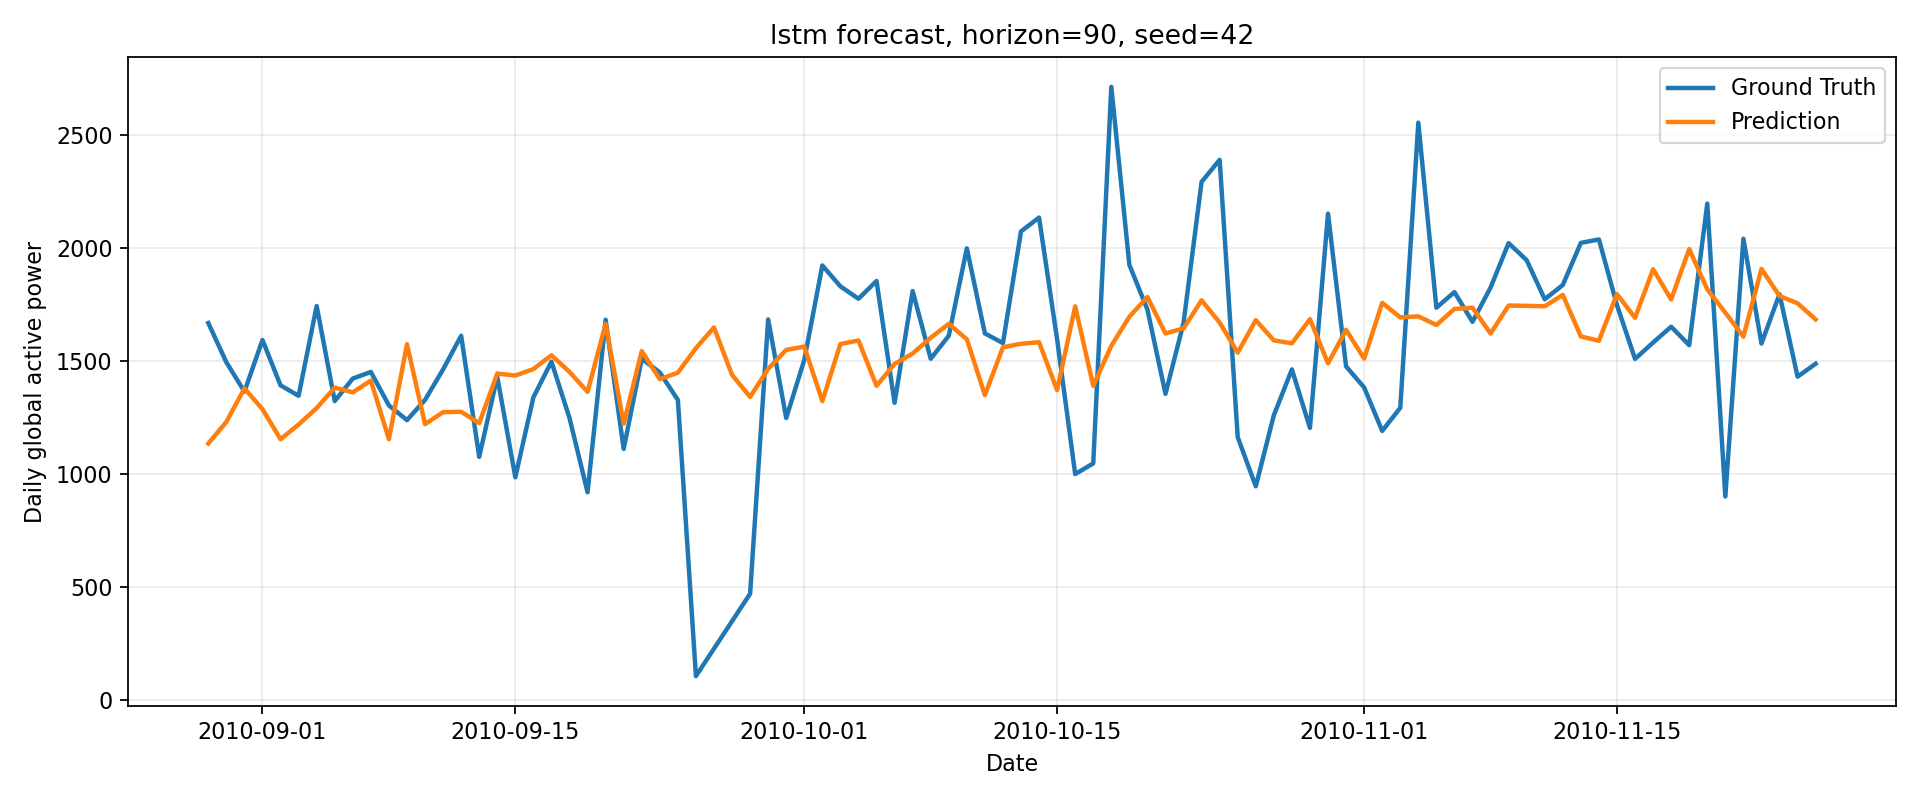
\includegraphics[width=\textwidth]{figures/lstm_h90_seed42.png}
  \caption{LSTM，未来 90 天}
\end{subfigure}
\begin{subfigure}{0.98\textwidth}
  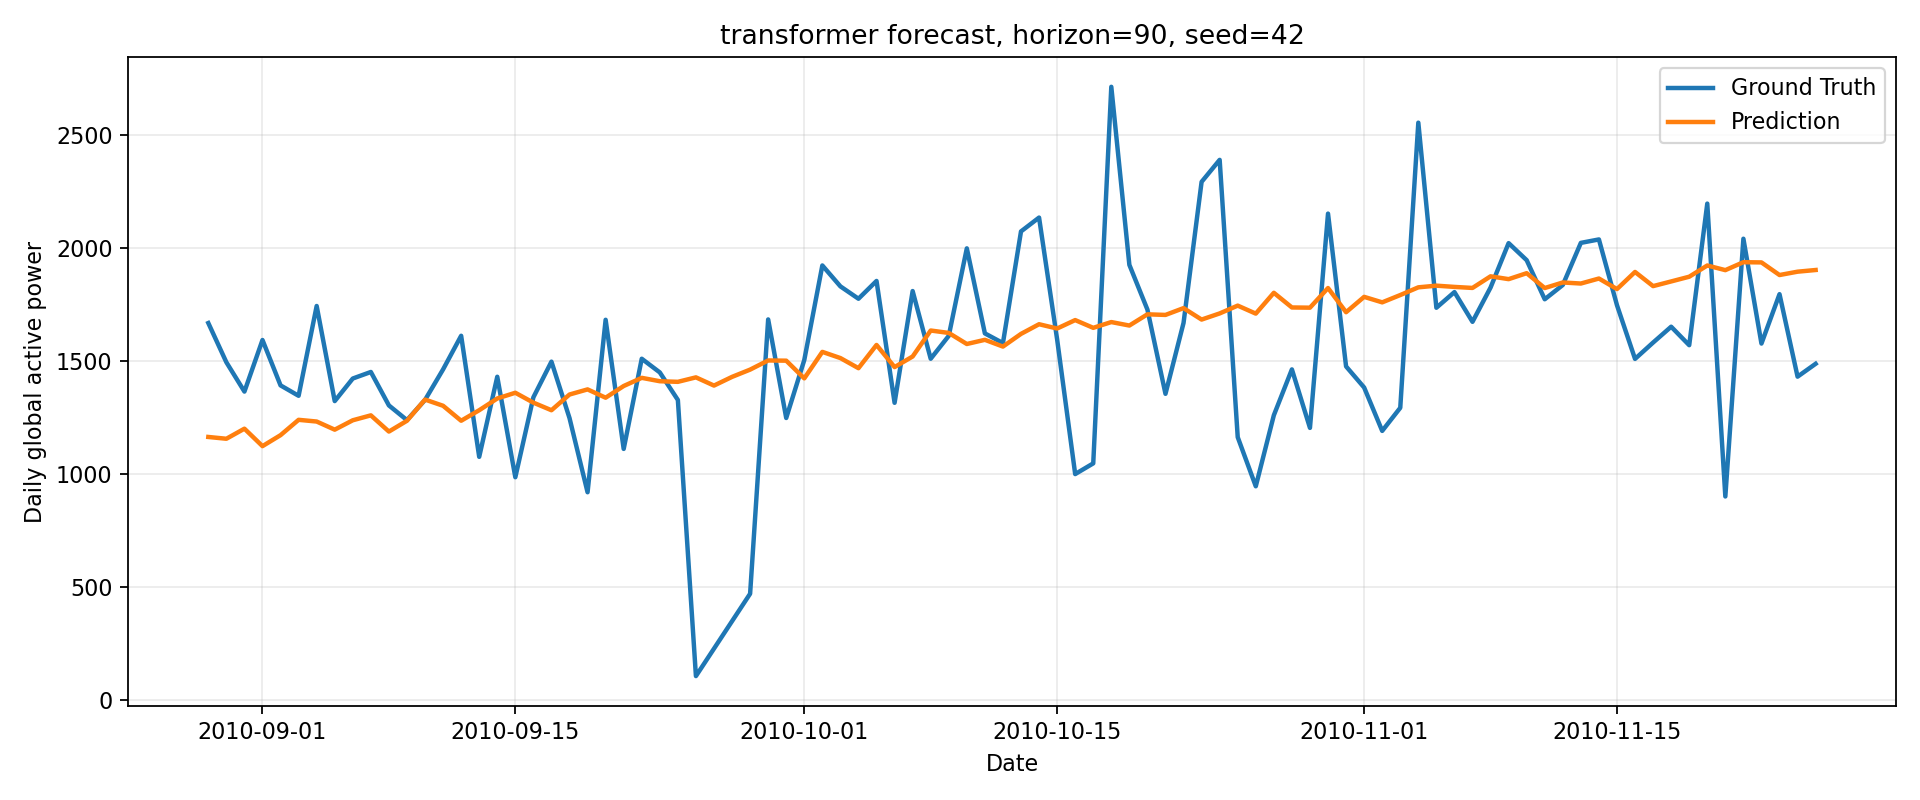
\includegraphics[width=\textwidth]{figures/transformer_h90_seed42.png}
  \caption{Transformer，未来 90 天}
\end{subfigure}
\begin{subfigure}{0.98\textwidth}
  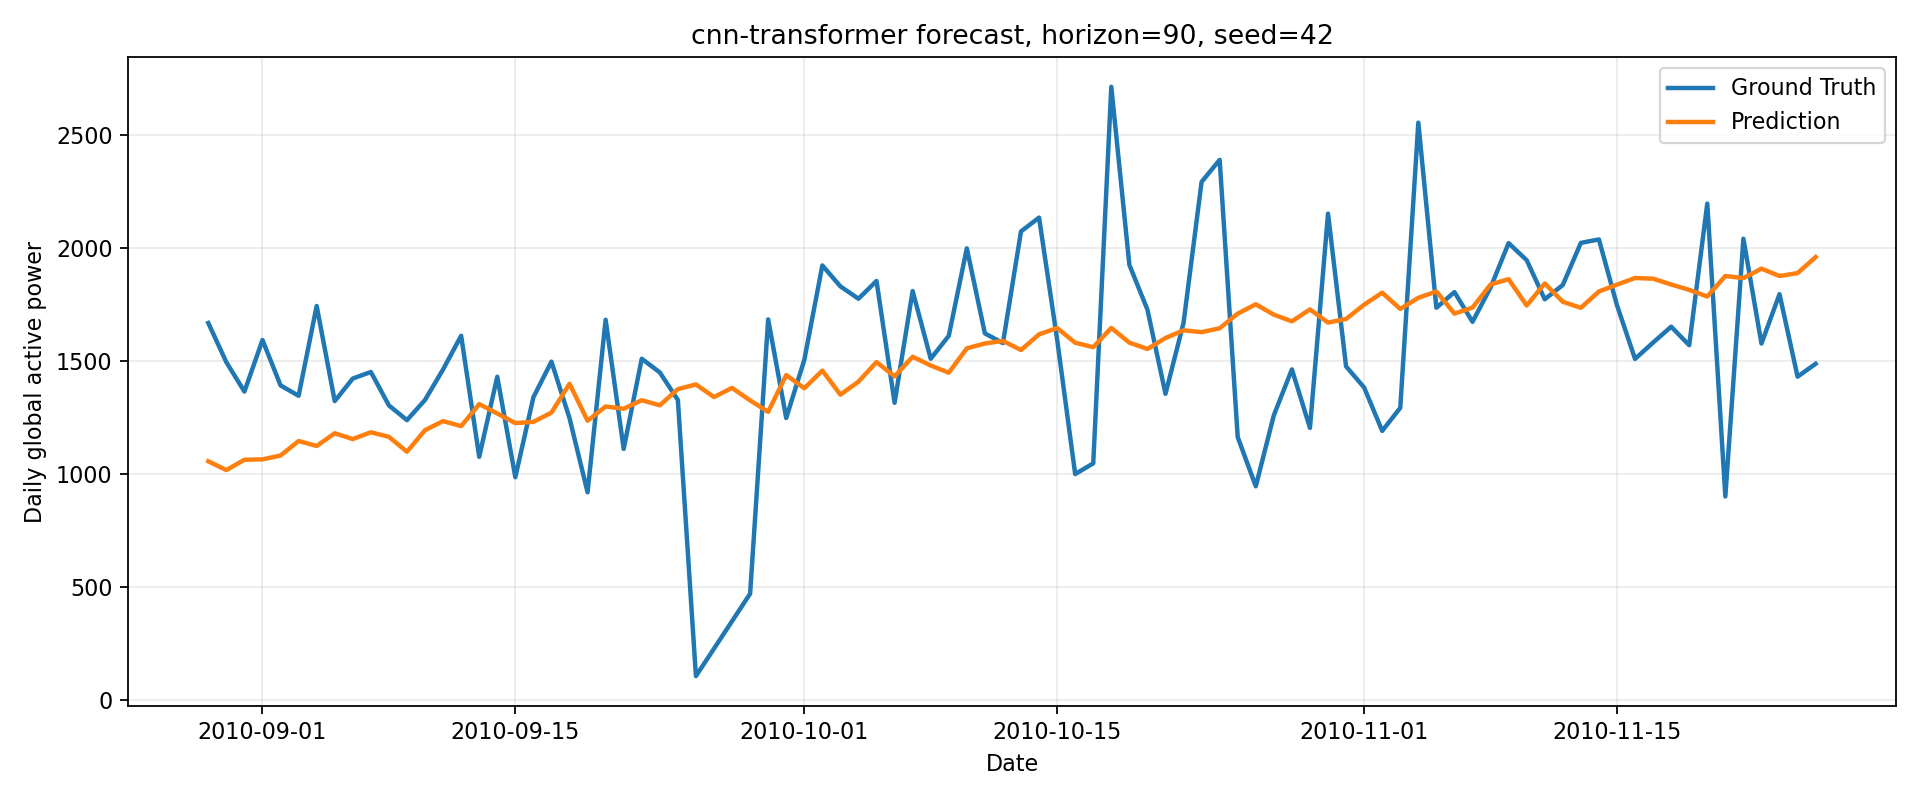
\includegraphics[width=\textwidth]{figures/cnn_transformer_h90_seed42.png}
  \caption{CNN-Transformer，未来 90 天}
\end{subfigure}
\caption{短期预测中预测值与真实值的对比曲线，展示 seed=42 的测试窗口结果。}
\end{figure}

短期预测中，Transformer 的 MSE 和 MAE 均最低，说明在加入月度气象特征后，自注意力结构对 90 天输入窗口中的多变量关系刻画更充分。LSTM 的标准差较小，表现仍然稳定，但平均误差略高于 Transformer。CNN-Transformer 的预测曲线整体较平滑，且 seed=44 的误差明显偏高，说明复杂结构在小规模日级样本上更容易受到初始化和训练稳定性的影响。三种模型都能学习总体用电水平，但对真实曲线中的尖峰和低谷响应不足，这些突发波动往往来自家庭成员作息、电器临时使用等行为因素，难以仅依靠月度天气变量准确解释。

\subsection{长期预测：未来 365 天}

\begin{table}[H]
\centering
\caption{未来 365 天预测结果}
\begin{tabular}{lrrrr}
\toprule
模型 & MSE mean & MSE std & MAE mean & MAE std \\
\midrule
Transformer & 163202.91 & 4906.76 & 305.77 & 5.66 \\
LSTM & 166359.99 & 2580.81 & 306.40 & 3.23 \\
CNN-Transformer & 166535.13 & 2551.06 & 306.41 & 1.66 \\
\bottomrule
\end{tabular}
\end{table}

\begin{figure}[H]
\centering
\begin{subfigure}{0.98\textwidth}
  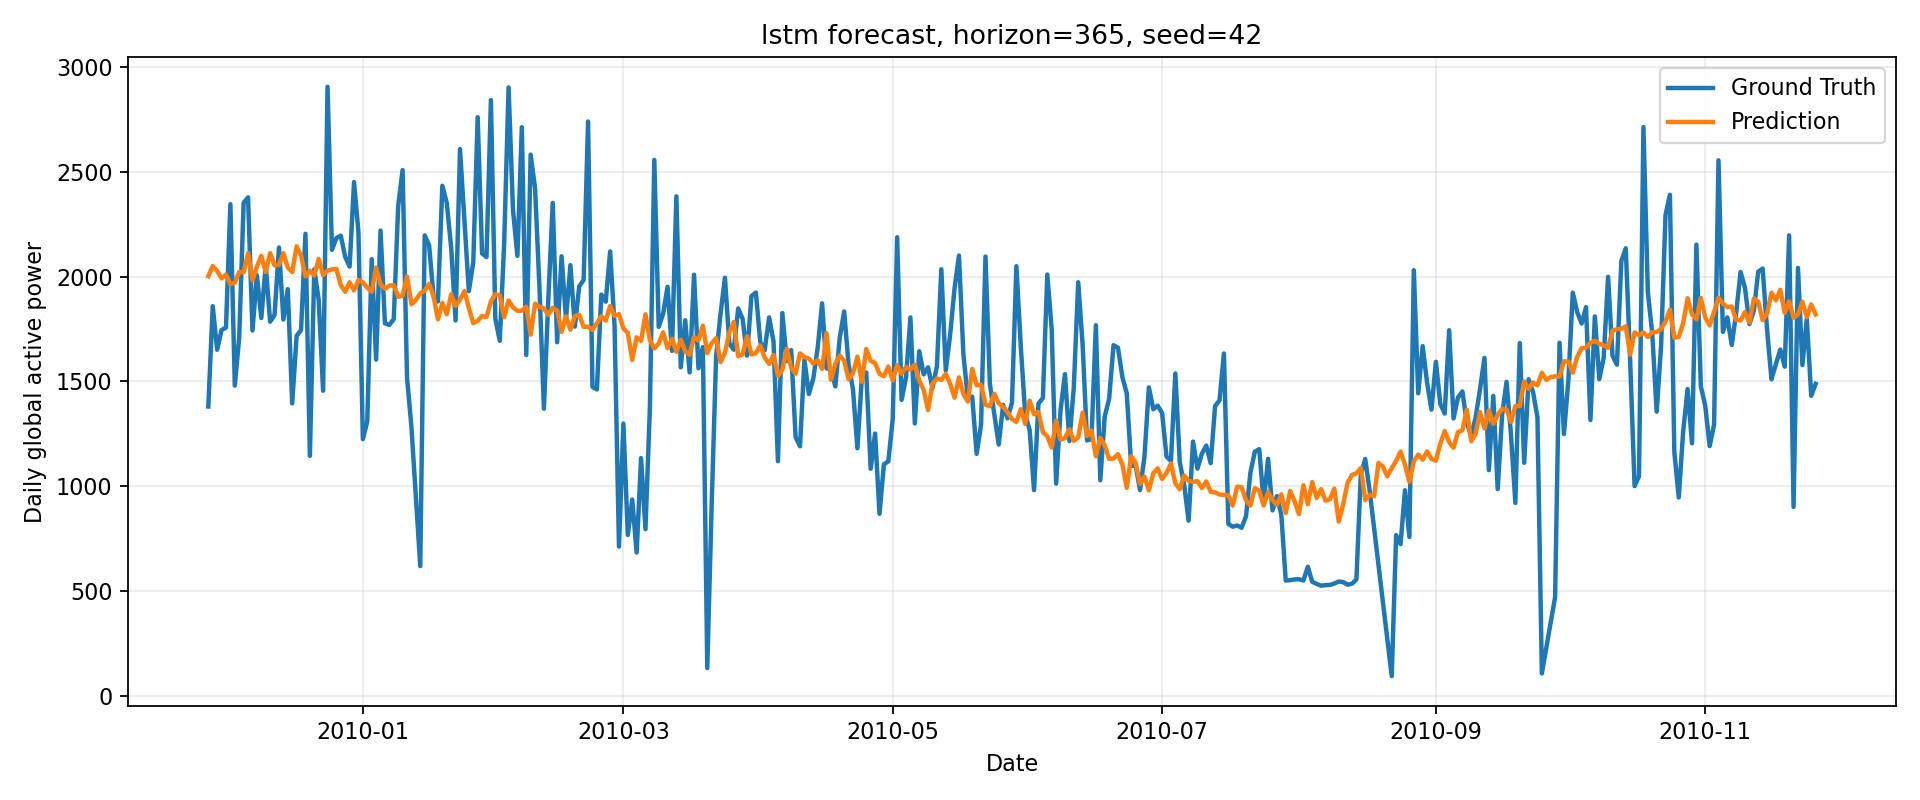
\includegraphics[width=\textwidth]{figures/lstm_h365_seed42.png}
  \caption{LSTM，未来 365 天}
\end{subfigure}
\begin{subfigure}{0.98\textwidth}
  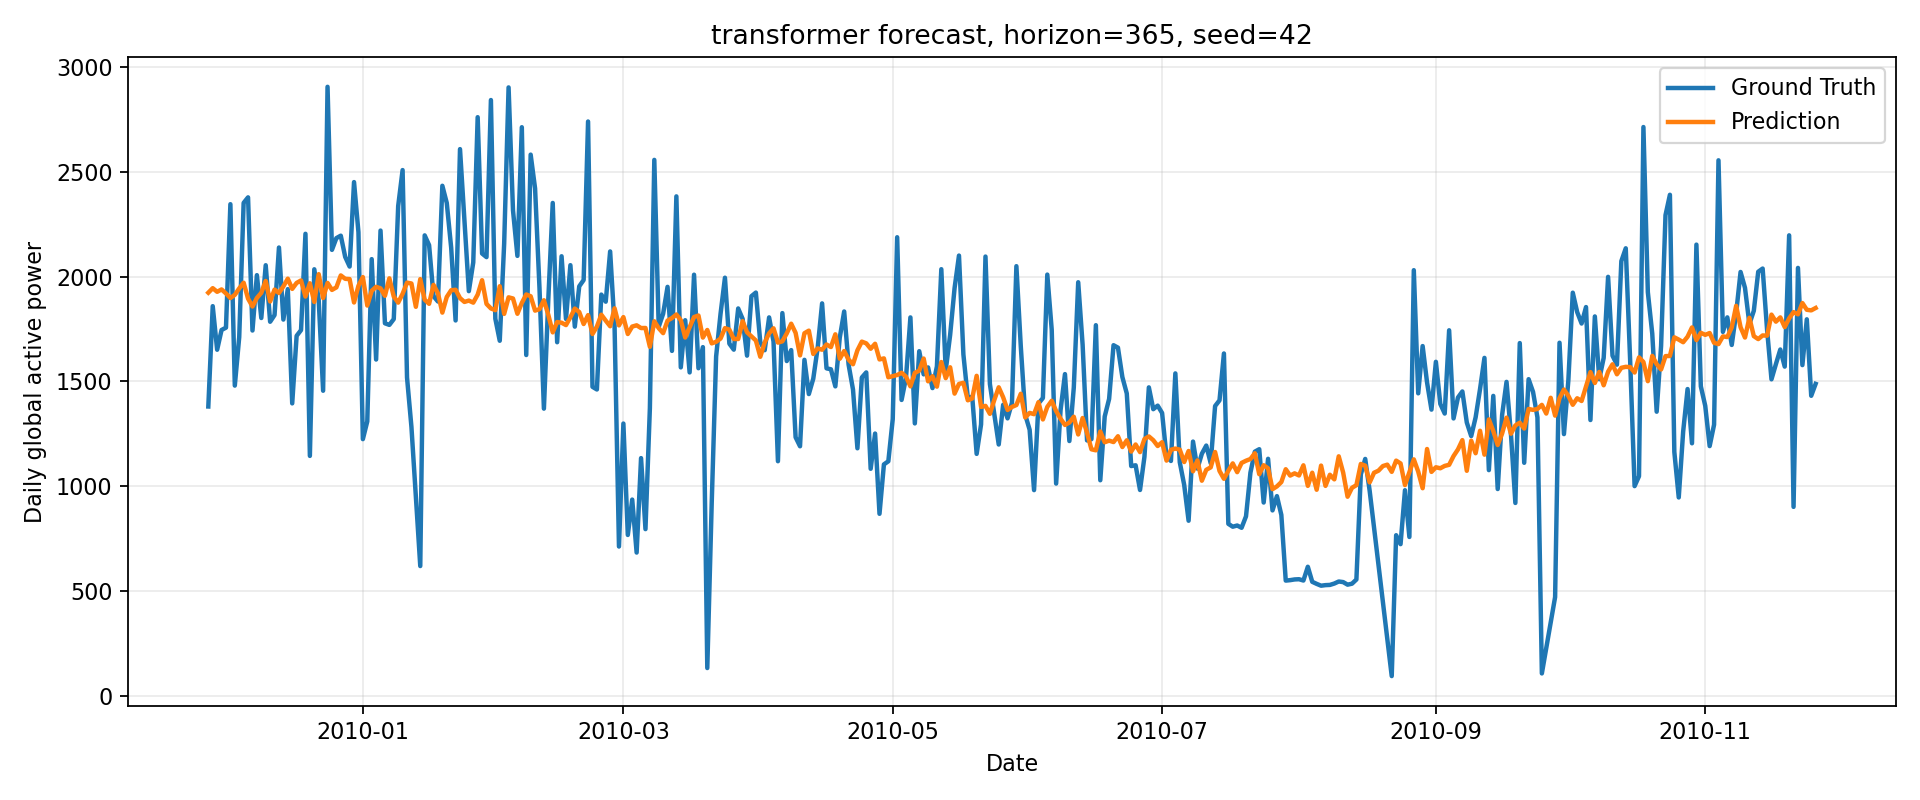
\includegraphics[width=\textwidth]{figures/transformer_h365_seed42.png}
  \caption{Transformer，未来 365 天}
\end{subfigure}
\begin{subfigure}{0.98\textwidth}
  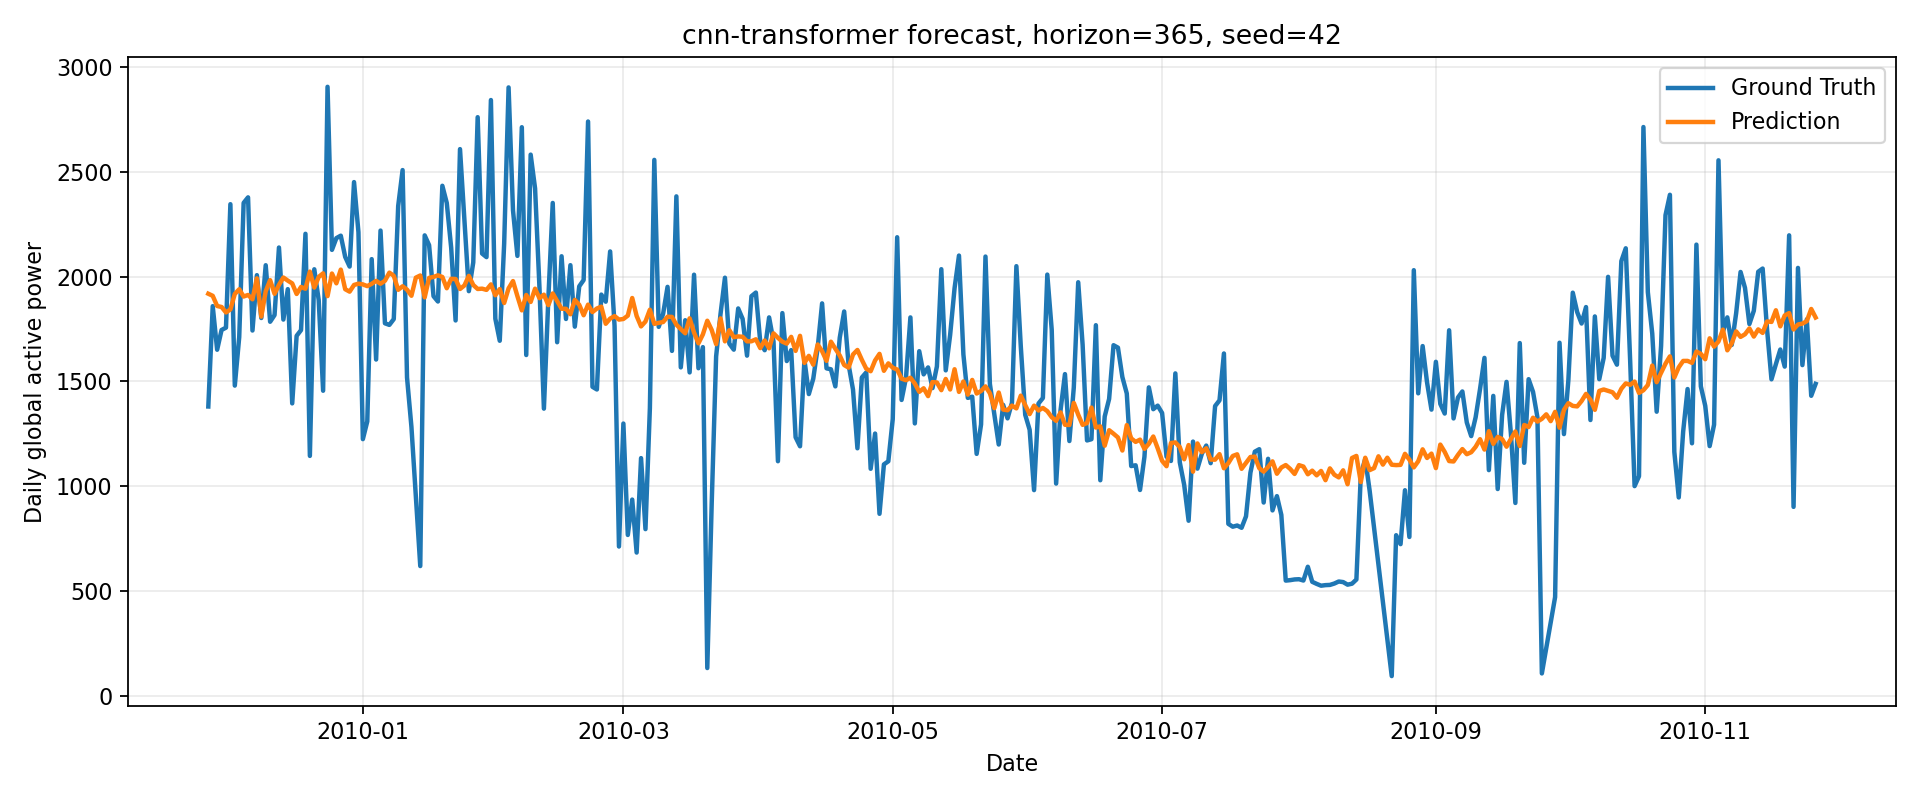
\includegraphics[width=\textwidth]{figures/cnn_transformer_h365_seed42.png}
  \caption{CNN-Transformer，未来 365 天}
\end{subfigure}
\caption{长期预测中预测值与真实值的对比曲线，展示 seed=42 的测试窗口结果。}
\end{figure}

长期预测中，Transformer 的 MSE 和 MAE 最低，说明自注意力机制在建模年尺度趋势方面仍然更有优势。从曲线可以观察到，模型能够学习到真实用电曲线中从冬季较高、夏季下降、秋冬回升的整体趋势。加入降水量、不同阈值降水日数和雾日数后，模型可以获得一定外部环境信息，但由于天气数据为月度粒度，并且本任务预测的是单个家庭每日总有功功率，三种模型仍然对日级随机波动和极端值预测不足，预测曲线明显比真实曲线平滑。这是多步直接预测任务中的常见现象：模型更容易学习平均趋势，而难以准确预测未来某一天的突发用电行为。

\subsection{三种方法比较}

综合两类任务可以看出，Transformer 在 90 天和 365 天预测中都取得了最低平均误差，说明其对多变量输入和较长预测区间具有较强适应性。LSTM 的表现接近 Transformer，且在部分指标上标准差较小，说明循环结构仍然是家庭负荷预测中的稳健基线。CNN-Transformer 作为改进模型具有清晰的结构动机，但在本实验中并未取得最优性能。可能原因包括：第一，日级数据仅 1,442 条，经过 90 天输入和 365 天输出窗口构造后，可用长期训练样本较少；第二，模型复杂度提升后需要更长训练或更细致的超参数搜索；第三，用电数据中的尖峰和低谷往往由家庭行为触发，月度天气变量只能提供较粗的环境背景。该结果也说明复杂结构并不一定总能优于更简单的时间序列模型，模型改进需要结合数据规模、任务长度和训练稳定性共同分析\cite{linear}。

\section{讨论}

本实验完成了从分钟级原始数据清洗、天级聚合、月度天气特征融合、滑动窗口构造到多模型训练和评估的完整流程。实验结果表明，Transformer 在短期和长期预测中均取得最低平均误差，说明自注意力机制对多变量输入和较长预测区间具有较强适应性；LSTM 的误差接近 Transformer，仍是稳定可靠的序列预测基线。

本实验也存在一些限制。首先，天气数据为月度粒度，虽然能够表达降水和雾天等外部环境，但无法反映每日温度、湿度或节假日等更细变化。其次，模型采用直接多步输出，虽然训练和比较方便，但容易产生平滑预测，难以捕捉极端波动。再次，受 CPU 训练时间限制，本实验使用 20 轮训练和早停策略，未进行大规模超参数搜索。

后续可以从三个方向改进：一是加入日级温度、湿度、节假日等更细粒度外部变量，提高对季节和行为变化的解释能力；二是尝试趋势-季节分解后再建模，降低原始序列波动带来的学习难度；三是为 CNN-Transformer 引入残差连接、多尺度卷积或更长训练轮数，使其局部特征提取能力更充分发挥。

\section*{使用说明}

本报告文字组织和代码结构使用 ChatGPT/Codex 辅助完成，实验结果由本人运行代码生成。

\section*{参考文献}
\begingroup
\renewcommand{\bibsection}{}
\begin{thebibliography}{99}
  \bibitem{uci} Hebrail G, Berard A. Individual Household Electric Power Consumption: UCI Machine Learning Repository Dataset[DB/OL]. 2006. \url{https://doi.org/10.24432/C58K54}.
  \bibitem{meteofrance-monthly} Météo-France. Données climatologiques de base - mensuelles[DB/OL]. data.gouv.fr, 2026. \url{https://www.data.gouv.fr/datasets/donnees-climatologiques-de-base-mensuelles}.
  \bibitem{residential-lstm} Kong W, Dong Z Y, Jia Y, et al. Short-Term Residential Load Forecasting Based on LSTM Recurrent Neural Network[J]. IEEE Transactions on Smart Grid, 2019, 10(1): 841--851. \url{https://doi.org/10.1109/TSG.2017.2753802}.
  \bibitem{tft} Lim B, Arik S O, Loeff N, et al. Temporal Fusion Transformers for Interpretable Multi-horizon Time Series Forecasting[J]. International Journal of Forecasting, 2021, 37(4): 1748--1764. \url{https://doi.org/10.1016/j.ijforecast.2021.03.012}.
  \bibitem{lstm} Hochreiter S, Schmidhuber J. Long Short-Term Memory[J]. Neural Computation, 1997, 9(8): 1735--1780. \url{https://doi.org/10.1162/neco.1997.9.8.1735}.
  \bibitem{attention} Vaswani A, Shazeer N, Parmar N, et al. Attention Is All You Need[C]//Advances in Neural Information Processing Systems. 2017, 30. \url{https://papers.nips.cc/paper/7181-attention-is-all-you-need}.
  \bibitem{informer} Zhou H, Zhang S, Peng J, et al. Informer: Beyond Efficient Transformer for Long Sequence Time-Series Forecasting[J]. Proceedings of the AAAI Conference on Artificial Intelligence, 2021, 35(12): 11106--11115. \url{https://doi.org/10.1609/aaai.v35i12.17325}.
  \bibitem{autoformer} Wu H, Xu J, Wang J, et al. Autoformer: Decomposition Transformers with Auto-Correlation for Long-Term Series Forecasting[C]//Advances in Neural Information Processing Systems. 2021, 34: 22419--22430. \url{https://proceedings.neurips.cc/paper/2021/hash/bcc0d400288793e8bdcd7c19a8ac0c2b-Abstract.html}.
  \bibitem{patchtst} Nie Y, Nguyen N H, Sinthong P, et al. A Time Series Is Worth 64 Words: Long-term Forecasting with Transformers[C]//International Conference on Learning Representations. 2023. \url{https://openreview.net/forum?id=Jbdc0vTOcol}.
  \bibitem{linear} Zeng A, Chen M, Zhang L, et al. Are Transformers Effective for Time Series Forecasting?[J]. Proceedings of the AAAI Conference on Artificial Intelligence, 2023, 37(9): 11121--11128. \url{https://doi.org/10.1609/aaai.v37i9.26317}.
\end{thebibliography}
\endgroup

\end{document}
